\documentclass{article}
\usepackage[utf8]{inputenc}
\usepackage[spanish]{babel}
\usepackage{listings}
\usepackage{graphicx}
\graphicspath{ {images/} }
\usepackage{cite}

\begin{document}

\begin{titlepage}
    \begin{center}
        \vspace*{1cm}
            
        \Huge
        \textbf{Proyecto De Investigación}
            
        \vspace{0.5cm}
        \LARGE
        Taller Memoria
            
        \vspace{1.5cm}
            
        \textbf{Juan Pablo Palacios Monsalve}
            
      
        
        \vspace{2.0cm}
        \textbf{Profesor: Augusto Salazar}
      
    
        \textbf{Materia: Informática II}
      
        \vfill
        
        \vspace{0.8cm}
     
        \Large
        Despartamento de Ingeniería Electrónica y Telecomunicaciones\\
        Universidad de Antioquia\\
        Medellín\\
        Septiembre de 2020
      
    \end{center}
\end{titlepage}

\tableofcontents
\newpage
\section{Introducción}\label{intro}
Dentro de los componentes de nuestros dispositivos inteligentes (computadoras, celulares, tabletas, etc.) se encuentra uno que se encarga de almacenar toda la información que se procesa de manera temporal, la memoria. Podemos pensar en ella como en un refrigerador lleno de toda clase comida (datos). Para que la memoria pueda funcionar, específicamente la de un computador, son indispensables algunos componentes como el external data bus (EDB), el cual se constituye de una fila de cables que interconectan las partes del computador, equiparándose así a las venas de nuestro cuerpo. Otro componente es el chip controlador de memoria (MCC), el cual es muy importante ya que es el puente directo entre la memoria y el procesador; de este modo, podríamos equiparar el MCC con un nervio de nuestro cerebro que se conecta a los recuerdos. De este modo, el procesador solicita al MCC las instrucciones, este se dirige a la memoria, toma los datos y los envía a través del EDB. Sin embargo, para que el MCC se conecte con el procesador, es importante el Adress Bus, el cual se encarga de dicha tarea. En resumen, para que la memoria funcione adecuadamente, debe ocurrir lo siguiente:
\vspace{0.2cm}
 
 ``El Addres bus se encarga de enviar la dirección de los datos, pero no los datos en sí, luego el MCC toma la dirección de los datos, busca los datos en la memoria y entonces los datos se envían a través del EDB hacía el procesador"\cite[Programs and hardware. 5:51]{Coursera}.

\begin{figure}[h]
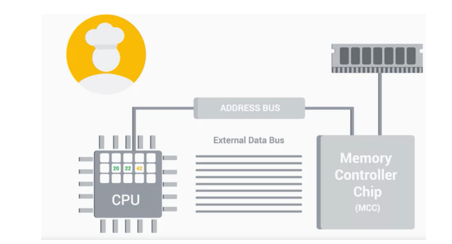
\includegraphics[width=10cm]{Captura.1.PNG}
\centering
\caption{Diagrama de comunicación entre la CPU y la memoria. Tomado de:\cite{Coursera}}
\label{Captura.1.PNG}
\end{figure}
Hay formas más rápidas de obtener datos para nuestro procesador y que este los procese. Por eso hablaré un poco más a fondo y de manera clara de la memoria, de su funcionalidad en sí y de sus tipos. 

\section{Contenido} \label{contenido}



\subsection{¿Qué es la memoria del computador?}
 ``En muchos sentidos, nuestros recuerdos nos representan, nos ayudan a recordar nuestro pasado, aprender y mantener habilidades, y planificar el futuro. Y para la computadora que actúa como una extensión de nosotros mismos, la memoria juega el mismo papel"\cite[How computer memory works. 00:06]{TEDwebsite}. 
\vspace{0.2cm}

De este modo, podemos decir que la memoria es un dispositivo para almacenar información a corto y largo plazo. A corto plazo, para tareas inmediatas, y a largo plazo, para tareas que requieran de un almacenamiento permanente.
Por otro lado, del mismo modo que los humanos tenemos diferentes lenguajes para comunicarnos, los computadores también tienen un lenguaje propio de comunicación, el cual consiste en comunicación binaria o sistema de numeración base 2, lo cual significa que se comunica únicamente mediante unos y ceros (bits); la memoria, tiene entonces como unidades básicas, los bits. Cada uno de estos ocupa un lugar en la denominada celda de memoria, que se compone de transistores y condensadores, cuyo estado solo puede variar en 1 y 0.  Toda la información que vemos en nuestras computadoras (videos, imágenes, texto) están compuestas de unos y ceros, lo cual significa que los archivos y programas contienen millones de bits que se encuentran procesados en la unidad de procesamiento central, equiparándose su función con la de nuestro cerebro. 
Al pulsar una tecla, puede ser un procesador de texto, por ejemplo, la CPU tomará la decisión de acceder a una de sus facetas mencionadas anteriormente, en este caso, a la memoria a corto plazo para recuperar los bits, los cuales puedes ser entendidos también como datos; el tiempo que se toma para realizar esta operación se conoce como “latencia de memoria”. Como las instrucciones para cada programa deben ser procesadas de manera continua y rápida, se tiene la libertad de acceder a cualquier espacio, en cualquier orden, dentro de la memoria a corto plazo, y de allí su nombre de Memoria de Acceso Aleatorio (RAM), cuya limitación más importante es que sólo puede almacenar datos mientras se tenga una fuente de alimentación.
\vspace{0.2cm}

Para que los datos no se pierdan una vez desaparezca la fuente de alimentación, hay que transferirlos en un dispositivo de almacenamiento a largo plazo, es decir, una memoria a largo plazo. De este tipo, existen tres principales:
\begin{itemize}
\item Almacenamiento magnético.
\item Almacenamiento óptico.
\item Unidades de estado sólido.
\end{itemize}
\subsection{Tipos de memoria}
\subsubsection{Memoria de acceso aleatorio (RAM)}
La memoria RAM es la se encargada del almacenamiento a corto plazo en los computadores, específicamente aquellos datos a los que queremos acceder de forma rápida y continua, lo cual quiere decir que los datos no son permanentes, sino que cambian constantemente. Al apagar la computadora, los datos almacenados se borran, lo que significa que la memoria RAM es de carácter volátil.

\begin{figure}[h]
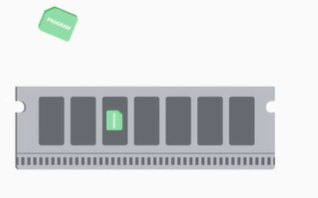
\includegraphics[width=8cm]{Captura.2.PNG}
\centering
\caption{La memoria RAM copia los programas. Tomado de:\cite{Coursera}}
\label{Captura.2.PNG}
\end{figure}
\subsubsection{Memoria dinámica de acceso aleatorio (DRAM)}
 La memoria DRAM se denomina dinámica porque retiene datos por un corto periodo de tiempo antes de perderlos, además, necesita cargarse y descargase con frecuencia para poder retener la información.\cite[How computer memory works. 2:07]{TEDwebsite}. También, tiene la capacidad de construir celdas con una gran densidad de posiciones y lograr que funcionen a altas velocidades, tanto así, que su latencia es muy baja (del orden de los 100 nanosegundos).

\begin{figure}[h]
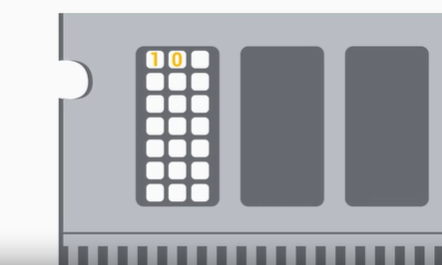
\includegraphics[width=5cm]{dram.PNG}
\centering
\caption{representada con 0 cuando no está cargada, 1 cuando lo está. \centering Tomado de:\cite{Coursera}}
\label{dram.PNG}
\end{figure}
\subsubsection{DRAM sincrónica}
Este tipo de memoria está sincronizada con la velocidad del reloj del sistema, es decir, la velocidad a la que la CPU realiza un ciclo de operaciones, lo que permite procesar más rápido los datos. Cabe resaltar que la SDRAM, es la memoria más rápida de un sistema operativo y ocupa más espacio que la DRAM.
\begin{figure}[h]
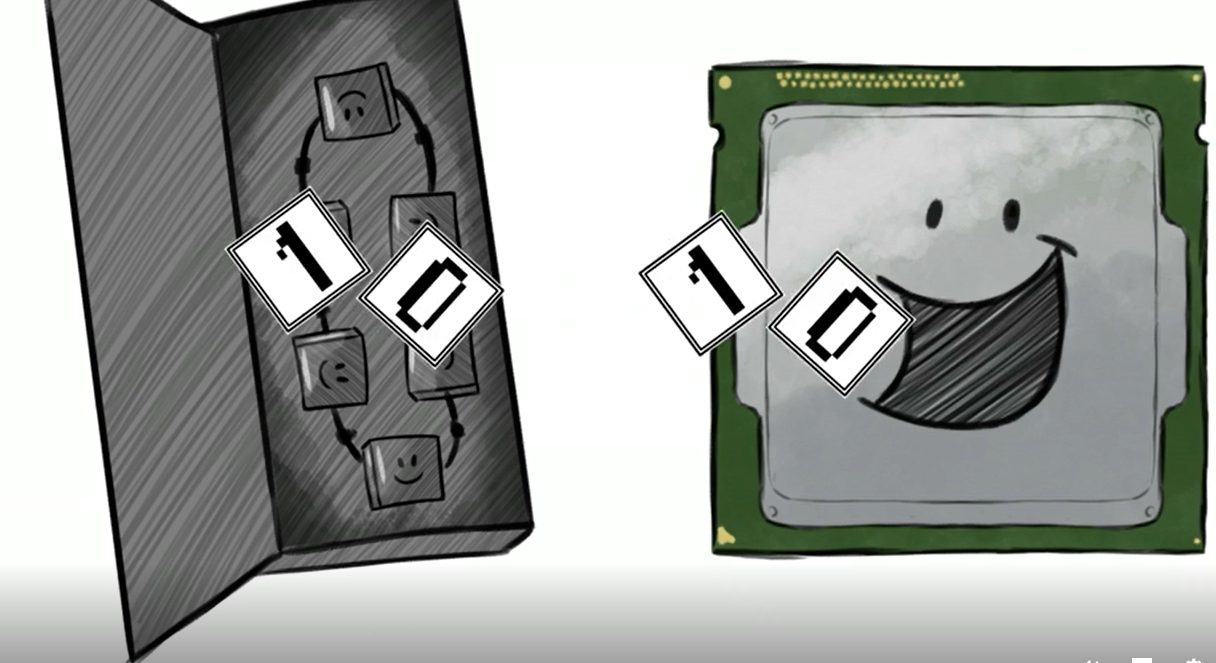
\includegraphics[width=8cm]{SDRAm.PNG}
\centering
\caption{Compuesta por 6 transistores entrelazados que no necesitan recarga. \centering Tomado de:\cite{TEDwebsite}}
\label{SDRAm.PNG}
\end{figure}
\subsubsection{SDRAM de doble velocidad de datos (DDR)}
La memoria DDR es una versión mejorada de la SDRAM, ya que es más rápida, consume menos energía y cuenta con mayor capacidad. Su versión más actual es la \textbf{DDR4}, un tipo de memoria a corto plazo que es la más rápida que hay disponible actualmente en el mercado; es decir, que los programas pueden ejecutarse a mayor rapidez y pueden ejecutarse más programas de forma simultánea.
\vspace{0.2cm}
\begin{figure}[h]
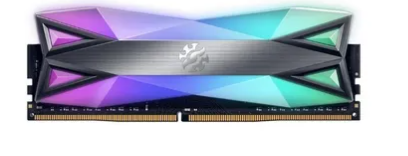
\includegraphics[width=8cm]{DDR4.PNG}
\centering
\caption{DDR4 Gaming RAM. Tomado de:\cite{mercadolibre}. }
\label{DDR4.PNG}
\end{figure}
\newpage
\subsubsection{Memoria cache}
La memoria caché está integrada a la CPU y es más pequeña que la RAM, sin embargo, permite almacenar los datos que se usan con más frecuencia, de forma similar a los bolsillos de un pantalón, en donde llevamos cosas de uso frecuente, como el celular, las llaves, la billetera, etc. Este tipo de memoria consta de tres niveles:
\begin{enumerate}
\item \textbf{L1}: La más rápida de todas.Su función principal es guardar datos importantes de uso frecuente (usuarios,contraseñas).
\item \textbf{L2}: Almacena información recientemente visitada (Sitios Web)
\item \textbf{L3}: Es una memoria especializada en ayudar a mejorar los rendimientos de los niveles L1 y L2.
\end{enumerate}

\begin{figure}[h]
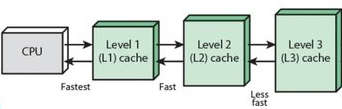
\includegraphics[width=6cm]{Cache.PNG}
\centering
\caption{Jerarquia de la memoria cache. \centering Tomado de:\cite{URUGUAYOC}}
\label{Cache.PNG}
\end{figure}
\subsubsection{Memoria ROM}
La memoria de sólo lectura (Read Only Memory) es una memoria, que como su nombre lo indica, es de solo lectura, es decir, se puede recuperar pero no intervenir ni modificar. Además, cumple unas tareas de suma importancia como el almacenamiento de software, de modo que impide que las personas lo alteren por error o se interrumpa su funcionamiento. Otra de sus tareas, consiste en el almacenamiento de datos, pero estos son datos que no requieren modificaciones, como los operadores matemáticos y lógicos, tablas de consulta, entre otros. Actualmente, este tipo de memoria se usa para instalar software de arranque como la BIOS (sistema básico de entrada y salida). 
\begin{figure}[h]
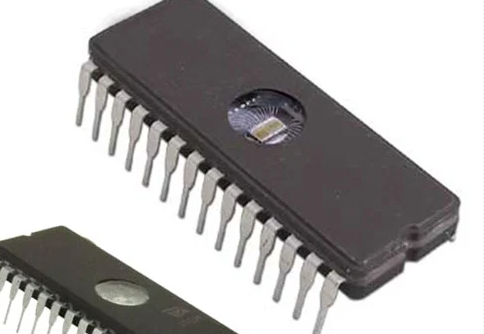
\includegraphics[width=4cm]{ROM.PNG}
\centering
\caption{Memoria ROM.}
\label{ROM.PNG}
\end{figure}

\subsubsection{Unidad de Disco duro (HDD)}
 La unidad de disco duro, también conocido como almacenamiento magnético, almacena los datos de acuerdo a un patrón magnético que consiste en un disco giratorio que se encuentra cubierto por una película magnética\cite[How computer memory works. 2:57]{TEDwebsite}), y un brazo mecánico que lee y escribe la información. Dicho disco gira a una velocidad, medida en revoluciones por minuto (RPM), que permite leer y escribir datos; por ejemplo, un disco duro de 500GB, tendría una velocidad aproximada de 5400RPM. La desventaja de estos discos es que son frágiles debido a sus partes móviles, ya que puede sufrir daños irreparables, y, por tanto, una pérdida de información valiosa.

\begin{figure}[h]
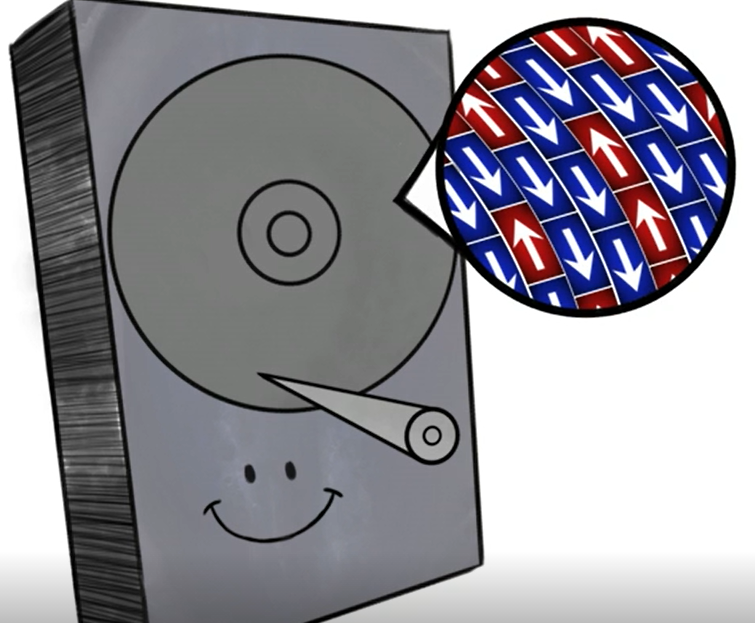
\includegraphics[width=4cm]{HDD.PNG}
\centering
\caption{Hard Drive Disk (HDD). \centering Tomado de: \cite{TEDwebsite}}.
\label{HDD.PNG}
\end{figure}
\subsubsection{Unidad de Disco duro de estado sólido (SDD)}
La SDD se asemeja al funcionamiento de las memorias USB, en cuanto a que la información se almacena en microchips, por tanto, los datos viajan a una velocidad superior que en los HDD; esto debido a que usan transistores de puerta flotante que almacenan datos atrapando o eliminando cargas eléctricas dentro de sus estructuras internas\cite[How computer memory works. 3:42]{TEDwebsite}. Al no tener parte móviles se disminuye el riesgo de daño y es más probable, que, si sufre un daño, se pueda salvar la información; sin embargo, la desventaja es que son muy costosos y cuentan con menor capacidad de almacenamiento, en comparación con los HDD.


\begin{figure}[h]
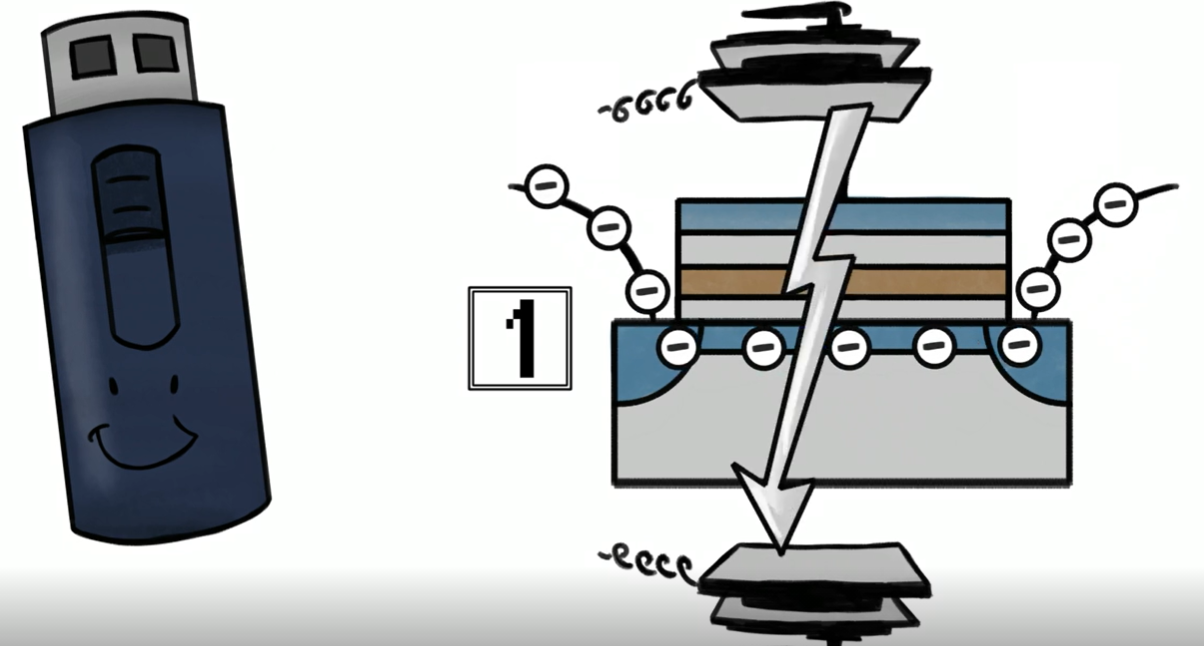
\includegraphics[width=5cm]{SDD.PNG}
\centering
\caption{transistores de puerta flotante de una SDD. Tomado de:\cite{TEDwebsite}}
\label{SDD.PNG}
\end{figure}
\newpage
\subsection{Gestión de memoria en un computador}
El sistema operativo (SO) es el encargado de llevar a cabo el proceso de gestión de memoria del computador, por medio de registros para destinar partes de la memoria a los programas que son requeridos en su momento, y a su vez, liberar partes de la misma que no se están usando para que se encuentren disponibles para su almacenamiento.
\vspace{0.2cm}

\textbf{Caracteristicas}:

\begin{itemize}
\item\textbf{Protección}: ``El principal propósito de la protección de memoria es evitar que un proceso en un sistema operativo acceda a la memoria que no le ha sido asignada"\cite[Unidad 3. Procesos de memoria y almacenamiento]{Sites.Google}.
\item\textbf{Memoria Compartida}:  ``Aunque la memoria utilizada por diferentes procesos suele estar protegida, algunos procesos puede que sí tengan que compartir información y, para ello, han de acceder la misma sección de memoria. La memoria compartida es una de las técnicas más rápidas para posibilitar la comunicación entre procesos"\cite[Unidad 3. Procesos de memoria y almacenamiento]{Sites.Google}.
\item\textbf{Organización Lógica}:  ``Permiten que los programas se escriban como módulos compilables y ejecutables por separado"\cite[Unidad 3. Procesos de memoria y almacenamiento]{Sites.Google}.
\item\textbf{Organización Física}:  ``La memoria suele dividirse en un almacenamiento primario de alta velocidad y uno secundario de menor velocidad.  La gestión de memoria del sistema operativo se ocupa de trasladar la información entre estos dos niveles de memoria"\cite[Unidad 3. Procesos de memoria y almacenamiento]{Sites.Google}.
\end{itemize}
\newpage
\subsection{¿Qué hace que una memoria sea más rapida que otra?
\centering¿Por qué esto es importante?}
Lo que genera que una memoria sea más rápida que otra son dos elementos muy importantes: \textbf{la frecuencia} y \textbf{la latencia}.La primera, se refiere a la velocidad de ciclos en un segundo, es decir, mientras más grande sea la frecuencia que tiene una memoria, más rápida será la cantidad de ciclos. La segunda, se puede entender como el retraso que experimenta la memoria.
\vspace{0.2cm}

Para conocer la velocidad exacta de la latencia se debe tener en cuenta un número importante que, multiplicado con la frecuencia, arroja con exactitud el llamado \textbf{cast latency}. El dato de frecuencia viene contramarcado en la parte trasera del módulo de memoria, sin embargo, ese no es valor verdadero. Los módulos más actuales y comunes son los DDR, cada uno tiene dos líneas de datos donde cada línea corre a la mitad de lo que dice el módulo, y esta sí es la frecuencia verdadera. Por ejemplo, si se tienen 3000 Mhz la frecuencia real será: 1500Mhz. Como se mencionó anteriormente, usando el cast de latencia y la frecuencia real podemos encontrar el tiempo de respuesta de nuestros módulos de memoria (velocidad de latencia), donde los mejores módulos cuentan con una velocidad aproximada de 10ns. Esto quiere decir que, mientras más nanosegundos haya, más lenta será la memoria.
\vspace{0.2cm}

En este sentido, la rapidez de una memoria es importante porque una mayor frecuencia permite tener transferencia de datos en menos tiempo. En procesos como producción y renderización, la velocidad de memoria es un apartado de suma importancia.

\begin{figure}[h]
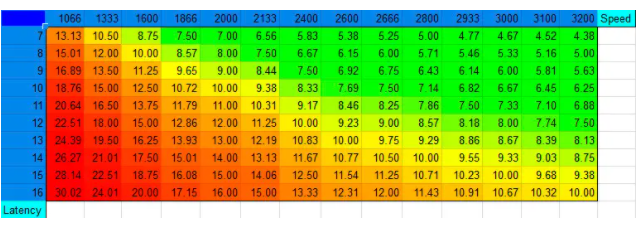
\includegraphics[width=12cm]{latencia.PNG}
\centering
\caption{Frecuencia vs latencia. Tomado de:\cite{Frecuencia}}
\label{latencia.PNG}
\end{figure}
\newpage
\section{Conclusión}
Se tiende a creer que la memoria es estable y duradera, sin embargo, puede degradarse con facilidad. Generalmente, la vida útil de estos dispositivos no supera los diez años; además, con los avances tecnológicos, diseñadores, diseñadores, científicos e ingenieros se enfrentan con barreras como tamaño, costo y velocidad, al intentar explotar al máximo las propiedades físicas de los materiales con la esperanza de crear dispositivos que cumplan con estos requerimientos, pero siempre teniendo que sacrificar algún otro apartado del hardware.
\vspace{0.2cm}

 ``Por ahora, la inmortalidad queda fuera del alcance, tanto para los seres humanos como para las computadoras"\cite[How computer memory works. 4:39]{TEDwebsite}.



\newpage
\bibliographystyle{IEEEtran}
\bibliography{references}

\end{document}
